\subsubsection{Arquitectura general del sistema}

La estructura se describe con el modelo C4 \cite{brown2018c4} en los niveles de contexto y de contenedores; el comportamiento y el despliegue, con UML \cite{omg2017uml}. Los componentes del agente conversacional se presentan en un apartado propio.

\paragraph{Diagrama de contexto}

El diagrama de contexto muestra el sistema como una caja central y los actores y sistemas externos que interactúan con él (Figura~\ref{fig:ob2_c4_contexto}). Los pacientes acceden solo a través de WhatsApp; el personal de la clínica, a través de la aplicación web.

\begin{figure}[H]
\centering
\IfFileExists{img/C4_Contexto.png}{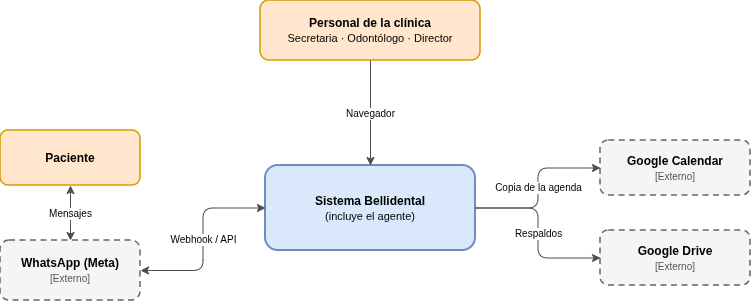
\includegraphics[width=0.95\linewidth]{img/C4_Contexto.png}}{\fbox{\parbox{0.9\linewidth}{\centering Pendiente: dibujar en draw.io según diagramas/drawio/ESPECIFICACION-arquitectura-general.md y exportar a img/C4\_Contexto.pdf}}}
\caption{Diagrama de contexto del sistema (C4, nivel 1)}
\label{fig:ob2_c4_contexto}
\end{figure}

\begin{table}[H]
\centering
\caption{Actores y sistemas externos del diagrama de contexto}
\label{tab:ob2_contexto}
\fontsize{9}{11}\selectfont
\renewcommand{\arraystretch}{1.2}
\setlength{\tabcolsep}{4pt}
\begin{tabularx}{\linewidth}{|>{\raggedright\arraybackslash}p{3.6cm}|>{\raggedright\arraybackslash}p{2.8cm}|>{\raggedright\arraybackslash}X|}
\hline
\textbf{Elemento} & \textbf{Tipo} & \textbf{Interacción} \\ \hline
Paciente & Persona & Agenda, reprograma o consulta por WhatsApp; recibe recordatorios si aceptó el aviso de privacidad en el agente \\ \hline
Secretaria & Persona & Gestiona la agenda, los pacientes y los cobros en la aplicación web \\ \hline
Odontólogo & Persona & Registra la historia clínica, el odontograma y los tratamientos \\ \hline
Director (administrador) & Persona & Administra los catálogos, los horarios y la configuración \\ \hline
WhatsApp Cloud API (Meta) & Sistema externo & Transmite los mensajes del paciente mediante un webhook y entrega las respuestas y los recordatorios \\ \hline
Google Calendar & Sistema externo & Recibe una copia de solo lectura de la agenda, con un calendario por profesional \\ \hline
Google Drive de la clínica & Sistema externo & Almacena los respaldos cifrados de la base de datos \\ \hline
\end{tabularx}
\end{table}

\paragraph{Diagrama de contenedores}

La aplicación web se ejecuta en el navegador de cada usuario; los demás contenedores se ejecutan en un único servidor virtual mediante Docker Compose (Figura~\ref{fig:ob2_c4_contenedores}). Un mismo nginx actúa como proxy inverso y sirve los archivos de la aplicación web. La API concentra la lógica del sistema, incluido el módulo del agente. El esquema de despliegue se detalla en un apartado posterior.

\begin{figure}[H]
\centering
\IfFileExists{diagramas/drawio/Contenedores_C4_2.png}{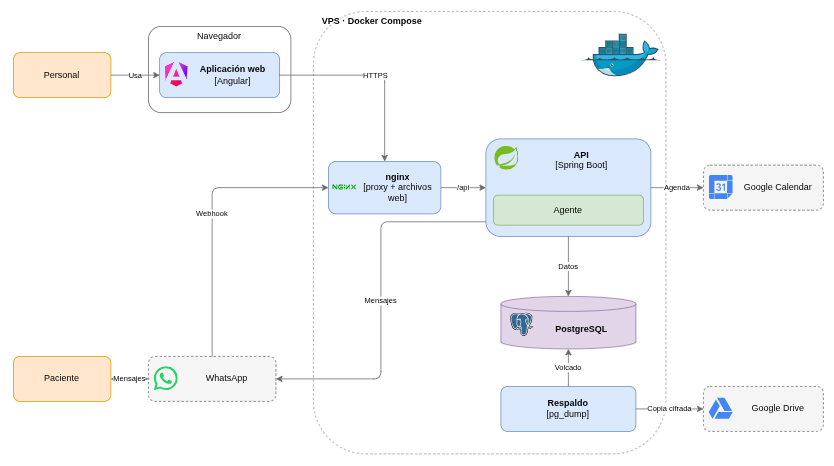
\includegraphics[width=\linewidth]{diagramas/drawio/Contenedores_C4_2.png}}{\fbox{\parbox{0.9\linewidth}{\centering Pendiente: dibujar en draw.io según diagramas/drawio/ESPECIFICACION-arquitectura-general.md y exportar a img/C4\_Contenedores.pdf}}}
\caption{Diagrama de contenedores del sistema (C4, nivel 2)}
\label{fig:ob2_c4_contenedores}
\end{figure}

\begin{table}[H]
\centering
\caption{Contenedores del sistema}
\label{tab:ob2_contenedores}
\fontsize{9}{11}\selectfont
\renewcommand{\arraystretch}{1.2}
\setlength{\tabcolsep}{4pt}
\begin{tabularx}{\linewidth}{|>{\raggedright\arraybackslash}p{3.2cm}|>{\raggedright\arraybackslash}p{3.8cm}|>{\raggedright\arraybackslash}X|}
\hline
\textbf{Contenedor} & \textbf{Tecnología} & \textbf{Responsabilidad} \\ \hline
Proxy inverso y servidor web & nginx con certificado de Let's Encrypt & Termina el cifrado en tránsito (TLS), sirve los archivos de la aplicación web y expone al exterior solo \texttt{/api} y el webhook de WhatsApp \\ \hline
Aplicación web & Angular 22.1, aplicación de una sola página & Se ejecuta en el navegador de la secretaria, el odontólogo y el director, sin instalación en los equipos \\ \hline
API del sistema & Spring Boot 3.5 con Java 21 & Lógica de negocio por módulos, autenticación con JWT y motor conversacional del agente \\ \hline
Base de datos & PostgreSQL 16 & Almacena los datos de la clínica en un esquema compartido e impide los cruces de citas \\ \hline
Servicio de respaldo & \texttt{pg\_dump} programado en Docker & Genera un volcado diario cifrado y lo copia a Google Drive \\ \hline
\end{tabularx}
\end{table}

\paragraph{Estilo arquitectónico: monolito modular}

La API se organiza como un monolito modular: una sola aplicación, desplegada como una unidad, cuyo código se divide en módulos por área funcional \cite{richards2020fundamentals}. Los antecedentes separan cada capacidad en un microservicio \cite{roca2020microservice,arcila2022microservice}. En una clínica pequeña, con un único desarrollador y un único servidor, esa separación añadiría despliegues, comunicación por red y monitoreo por servicio, una complejidad sin beneficio proporcional. De \cite{roca2020microservice} se conserva la idea de añadir capacidades sin modificar el núcleo, y de \cite{arcila2022microservice}, la autenticación con JWT.

La Figura~\ref{fig:ob2_modulos} agrupa los módulos esenciales y muestra cómo se comunican. La Tabla~\ref{tab:ob2_modulos} resume qué hace cada uno.

\begin{figure}[H]
\centering
\begin{tikzpicture}[
    font=\footnotesize, >={Stealth[length=2mm]},
    grupo/.style={draw, rounded corners=4pt, line width=0.8pt, align=center, inner sep=6pt, text width=#1},
    flecha/.style={->, draw=black!65, line width=0.6pt},
    evento/.style={->, draw=black!65, line width=0.6pt, dashed},
    et/.style={font=\scriptsize, fill=white, inner sep=1.5pt}
]
    \node[grupo=3.9cm, fill=dSistemaF, draw=dSistemaB] (agenda) at (0,2.7)
        {\textbf{Agenda}\\[2pt] Citas y regla anticruce\\ Copia en Google Calendar};
    \node[grupo=3.9cm, fill=dSistemaF, draw=dSistemaB] (base) at (0,0)
        {\textbf{Base}\\[2pt] Identidad y acceso\\ Pacientes\\ Profesionales y horarios};
    \node[grupo=3.5cm, fill=dClinicoF, draw=dClinicoB] (clin) at (5.0,1.35)
        {\textbf{Clínico y cobros}\\[2pt] Historia y atención\\ Odontograma\\ Tratamientos y recetas\\ Cobros};
    \node[grupo=2.6cm, fill=dAgenteF, draw=dAgenteB] (agente) at (-5.6,1.35)
        {\textbf{Agente}\\[2pt] Conversación\\ por WhatsApp\\ Recordatorios};

    \draw[flecha] (agenda) -- node[et] {usa} (base);
    \draw[flecha] ([yshift=8pt]clin.west) -- node[et] {usa} (agenda.east);
    \draw[flecha] ([yshift=-8pt]clin.west) -- node[et] {usa} (base.east);
    \draw[flecha] ([yshift=14pt]agente.east) -- node[et, sloped, above=1pt, fill=none] {agenda citas} ([yshift=4pt]agenda.west);
    \draw[evento] ([yshift=-6pt]agenda.west) -- node[et, sloped, below=1pt, fill=none] {eventos de cita} ([yshift=4pt]agente.east);
    \draw[flecha] ([yshift=-12pt]agente.east) -- node[et, sloped, below=1pt, fill=none] {identifica} (base.west);

    \node[font=\scriptsize\itshape, text=black!70, align=center, below=3pt of agente] {Sin acceso a datos\\clínicos (RNF03)};

    \node[draw=dExternoB, dashed, fill=dExternoF, rounded corners=3pt, minimum height=0.6cm,
          minimum width=13.6cm, font=\footnotesize\bfseries] at (0,-1.6) {Base de datos compartida (PostgreSQL)};

    \draw[flecha] (-6.8,-2.35) -- ++(0.8,0) node[right, font=\scriptsize, text=black] {llamada por interfaz pública};
    \draw[evento] (-1.4,-2.35) -- ++(0.8,0) node[right, font=\scriptsize, text=black] {evento de dominio};
\end{tikzpicture}
\caption{Módulos esenciales de la API y su comunicación}
\label{fig:ob2_modulos}
\end{figure}

\begin{table}[H]
\centering
\caption{Módulos esenciales del monolito modular}
\label{tab:ob2_modulos}
\fontsize{9}{11}\selectfont
\renewcommand{\arraystretch}{1.2}
\setlength{\tabcolsep}{4pt}
\begin{tabularx}{\linewidth}{|>{\raggedright\arraybackslash}p{3.6cm}|>{\raggedright\arraybackslash}X|>{\raggedright\arraybackslash}p{2.2cm}|}
\hline
\textbf{Módulo} & \textbf{Qué hace} & \textbf{Requerimiento} \\ \hline
Identidad y acceso & Usuarios, roles e inicio de sesión & RNF01 \\ \hline
Pacientes y profesionales & Datos de identificación, profesionales y horarios & RF06, RF07 \\ \hline
Agenda & Citas sin cruces, reprogramación y copia en Google Calendar & RF07, RF11, RF12 \\ \hline
Clínico & Historia clínica, odontograma, tratamientos y recetas & RF01 a RF05 \\ \hline
Cobros & Abonos y saldo por sesión & RF08 \\ \hline
Agente & Conversación por WhatsApp, aviso de privacidad y recordatorios & RF09 a RF14 \\ \hline
\end{tabularx}
\end{table}

Cada módulo expone una interfaz pública y no accede al interior de los demás. Los cambios de la agenda, como crear o reprogramar una cita, se publican como eventos que alimentan la copia en Google Calendar y los recordatorios. Así, un cambio en las reglas de agendamiento no altera la conversación del agente (Tabla~\ref{tab:ob2_atributos}). La auditoría (RNF02) es transversal y no forma un módulo. La separación no es completa: los módulos comparten la base de datos, de modo que un cambio de tabla puede afectar a más de uno.
